\documentclass[xcolor=dvipsnames, aspectratio = 169]{beamer}
\usepackage[english]{babel} %% english
\usepackage[utf8]{inputenc}
\usepackage[T1]{fontenc}
\usepackage{include/chariteBeamer}
\usepackage{hyperref}
\usepackage{blkarray}
\author[E. Sprünken]{Erin Sprünken}
\institute[]{
Institut für Biometrie und Klinische Epidemiologie\\[1Ex] 
Charité - Universitätsmedizin Berlin, Berlin\\[1Ex]
erin-dirk.spruenken@charite.de} 
\titlegraphic{\pgfuseimage{frontUnilogo}}

\tikzset{>=latex}
%\usepackage{amsmath}
%\usetikzlibrary{shadows}
\usepackage[edges]{forest}
\usetikzlibrary{positioning}
\usepackage{biostat}
\setbeamertemplate{caption}[numbered]
\let\qed\relax
\forestset{declare toks={elo}{}}
\graphicspath{{figures/}}
%% ================================================================== %% 

\author[L. Mödl, M. Becher, E. Sprünken]{Lukas Mödl, Matthias Becher, Erin Sprünken} 
\title{R-Kurs: Tag 3} 
\date[]{\today}

%% ================================================================== %% 
\setbeamercolor*{mycol}{bg=chariteGray, fg=chariteBlue}

\hyphenation{Sam-ples}
\begin{document}

%% ================================================================== %%
%% ================================================================== %%
\setbeamertemplate{footline}{\begin{tikzpicture}
    \node [inner sep=0pt, anchor=east] (0,0) {
      
\includegraphics[width=\paperwidth,height=0.7cm]{include/charite_footer}};
    \node [inner sep=0pt, anchor=east] at (-0.5ex,-0ex){};
\end{tikzpicture}}

\setbeamertemplate{headline}{
%\leavevmode
\hspace{-0.49em}\hbox{
	\begin{beamercolorbox}[wd=1.02\paperwidth,ht=2.25ex,dp=1ex,left]{mycol}%
    \usebeamerfont{section in head/foot}
  \end{beamercolorbox}%
}}
{
  \usebackgroundtemplate{ \hspace{-0.5em}\begin{tikzpicture}
  \node[opacity=0.7, anchor=south] (0,0) {
\includegraphics[height=\paperheight, width=1.04\paperwidth]{include/frontmatter.pdf}};
  \end{tikzpicture}
} 
%\frame{\titlepage}
\begin{frame}
\centering
	\vspace{4em}
	{\Large \textcolor{chariteBlue}{\inserttitle}}\\
	 \vspace{1em}
	{\Large \textcolor{black}{\insertauthor \\}} 
	\vspace{2em}
	{\footnotesize \textcolor{black}{\insertinstitute \\\vspace{1em} \insertdate}} 
	\vspace{0em}
	\begin{figure}[h!]
		
\includegraphics[width=5cm]{include/Charite_Logo.png}
	\end{figure}
%	\pgfuseimage{frontUnilogo}
\end{frame}
}
%% ================================================================== %%

\setbeamertemplate{footline}{\begin{tikzpicture}
    \node [inner sep=0pt, anchor=east] (0,0) {
      
\includegraphics[width=\paperwidth,height=0.7cm]{include/charite_footer}};
    \node [inner sep=0pt, anchor=east] at (-0.5ex,-0ex) {\tiny \insertframenumber{}$\,$|$\,$\inserttotalframenumber};
\end{tikzpicture}}

\setbeamertemplate{headline}{%
%\leavevmode%
\hspace{-0.49em}\hbox{
	\begin{beamercolorbox}[wd=.68\paperwidth,ht=2.25ex,dp=1ex,left]{mycol}%
    \usebeamerfont{section in head/foot}\hspace*{1em}
  \end{beamercolorbox}%
  \begin{beamercolorbox}[wd=.20\paperwidth,ht=2.25ex,dp=1ex,right]{mycol}%
    \usebeamerfont{author in head/foot}\insertshortauthor
  \end{beamercolorbox}%
  \begin{beamercolorbox}[wd=.14\paperwidth,ht=2.25ex,dp=1ex,center]{mycol}%
    \usebeamerfont{date in head/foot}\insertdate
  \end{beamercolorbox}%
  }
}


\frame{\tableofcontents}

\setbeamertemplate{headline}{%
%\leavevmode%
\hspace{-0.49em}\hbox{
	\begin{beamercolorbox}[wd=.68\paperwidth,ht=2.25ex,dp=1ex,left]{mycol}%
    \usebeamerfont{section in head/foot}\hspace*{1em}\thesection. \  \insertsectionhead
  \end{beamercolorbox}%
  \begin{beamercolorbox}[wd=.20\paperwidth,ht=2.25ex,dp=1ex,right]{mycol}%
    \usebeamerfont{author in head/foot}\insertshortauthor
  \end{beamercolorbox}%
  \begin{beamercolorbox}[wd=.14\paperwidth,ht=2.25ex,dp=1ex,center]{mycol}%
    \usebeamerfont{date in head/foot}\insertdate
  \end{beamercolorbox}%
  }
}

\section{Statistische Tests}

\begin{frame}[fragile]{Statistische Tests in R}
	\begin{itemize}
		\item t-Test = \verb+t.test()+
		\item Chi-Quadrat Test = \verb+chisq.test()+
		\item Wilcoxon-Mann-Whitney-Test = \verb+wilcox.test()+
		\item Fisher Test = \verb+fisher.test()+
		\item McNemar's Test = \verb+mcnemar.test()+
		\item Binomial Test = \verb+binom.test()+
		\item ...
	\end{itemize}
\end{frame}


\begin{frame}[fragile]{t-Test}
\verb+t.test(x,...)+\\
Parameter:
	\begin{itemize}
		\item x = Ein Vektor mit Daten
		\item y = Ein optionaler Vektor mit Daten, falls man zwei Gruppen vergleichen möchte
		\item alternative = c("two.sided", "less", "greater")
		\item mu = Der angenommene Mittelwert unter der Nullhypothese
		\item paired = c(TRUE, FALSE)
	\end{itemize}
\end{frame}

\begin{frame}[fragile]{Beispiel t-Test:}	
	\begin{center}
		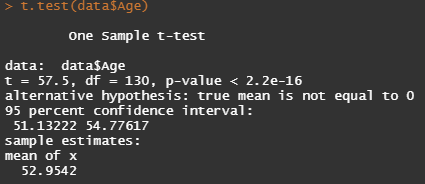
\includegraphics{OneSampleTtest}
	\end{center}
\end{frame}

\begin{frame}[fragile]{Beispiel t-Test:}	
	\begin{center}
		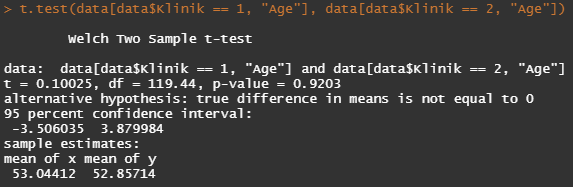
\includegraphics{TwoSampleTtest}
	\end{center}
Anmerkung: Per default nimmt R beim Zwei-Stichproben-t-Test ungleiche Varianz an
\end{frame}

\begin{frame}[fragile]{Chi-Quadrat Test:}	
	\verb+chisq.test()+ \\

	Beispiel: \\
	\begin{columns}[T]
		\begin{column}{0.5\textwidth}
			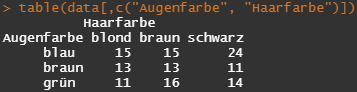
\includegraphics[width=7.5cm]{tabledata}
		\end{column}
		\begin{column}{0.5\textwidth}
			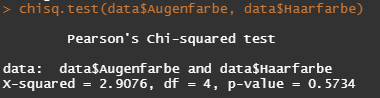
\includegraphics[width=7.5cm]{chisq}
		\end{column}
	\end{columns}
\end{frame}


%% ================================================================== %%
\section{Regressionsanalysen}

\begin{frame}[fragile]{Formeln in R}
	Um eine Regression durchzuführen müssen wir der Funktion sagen, welche Spalten in unseren Daten die unabhängigen Variablen sind und welche Spalte die abhängige Variable ist. Dafür gibt	es in R die Formelschreibweise:
	\begin{itemize}
		\item Nur bestimmte Variablen sollen in der Regression verwendet werden:
			\begin{center}
				Y\textasciitilde X1 + X2 + X3 + ... 
			\end{center}
		\item Alle Variablen im Datensatz sollen in der Regression verwendet werden:
			\begin{center}
				Y\textasciitilde.
			\end{center}
	\end{itemize}
\end{frame}



\begin{frame}[fragile]{Lineare Regression}
	\begin{itemize}
		\item \verb"model <- lm(Weight~Age+Sex+Height+Klinik, data =data)"
		\item \verb+summary(model)+
		\item Anmerkung: "0 +" am Anfang der Formel führt zu einer Regression ohne Intercept 
	\end{itemize}
			
	\begin{center}
		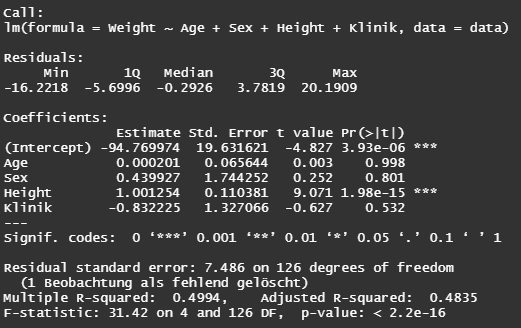
\includegraphics[height=3.75cm]{LinearRegressionSummary}
	\end{center}
\end{frame}

\begin{frame}[fragile]{Lineare Regression Plot}
	\begin{columns}[T]
		\begin{column}{0.6\textwidth}
			\begin{itemize}
				\item \verb+plot(data$Height,data$Weight)+
				\item \verb+abline(model)+
			\end{itemize}
		\end{column}
		\begin{column}{0.4\textwidth}
			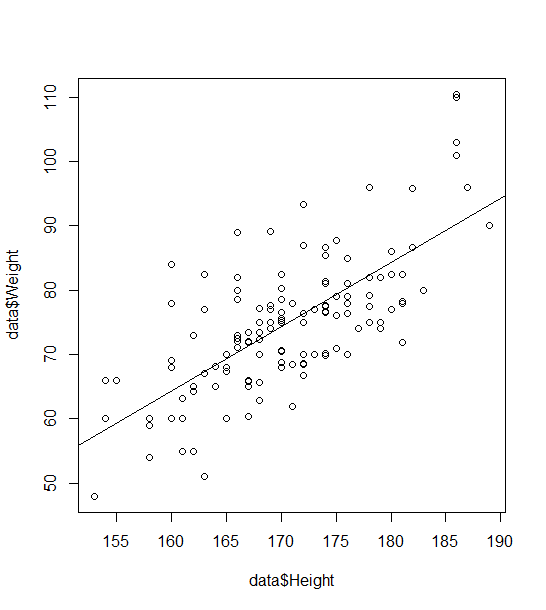
\includegraphics[height=6.5cm]{LinearRegressionPlot}
		\end{column}
	\end{columns}
\end{frame}

\begin{frame}[fragile]{Logistische Regression}
	\begin{itemize}
		\item \verb+model <- glm(y~., data = logistic_data, family = binomial)+
		\item \verb+summary(model)+
	\end{itemize}
			
	\begin{center}
		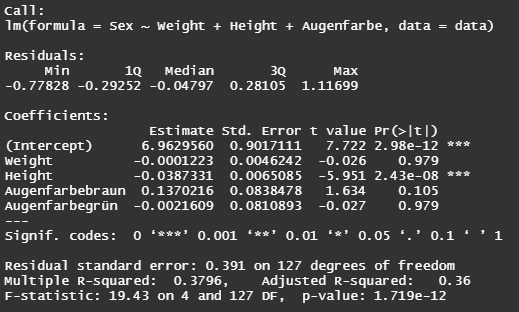
\includegraphics[height=4cm]{LogisticRegressionSummary}
	\end{center}
\end{frame}

\begin{frame}[fragile]{One-Way ANOVA}
	\begin{itemize}
		\item \verb+model <- aov(formula, data)+
	\end{itemize}	
	\begin{center}
		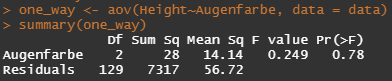
\includegraphics{OneWay}
	\end{center}
\end{frame}

\begin{frame}[fragile]{Two-Way ANOVA}
	\begin{center}
		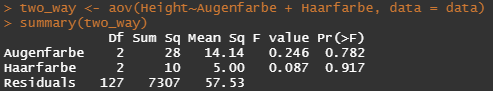
\includegraphics{TwoWay}
	\end{center}
\end{frame}

\begin{frame}[fragile]{Interaction ANOVA}
	\begin{center}
		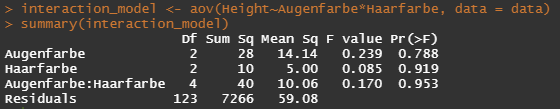
\includegraphics{Interaction}
	\end{center}
\end{frame}




%% ================================================================== %%

	


\section{\textsf R Pakete}


\begin{frame}[fragile]{Installation weiterer \textsf R Pakete}
    Jede \textsf R Umgebung installiert und lädt standardmäßig die Pakete \texttt{base}, \texttt{stats}, \texttt{datasets}, \texttt{methods} und \texttt{graphics}.\bigskip
    \begin{itemize}
        \item Installation weiterer Pakete mit:
        \begin{verbatim}
        install.packages("name-des-pakets", dependencies = TRUE)
        \end{verbatim}
        \item Bei jedem Start von \textsf R muss das Paket, wenn es verwendet werden soll, geladen werden:
        \begin{verbatim}
        library("name-des-pakets")
        \end{verbatim}
        \item Aktualisieren der Pakete mit:
        \begin{verbatim}
        update.packages()
        \end{verbatim}
    \end{itemize}
\end{frame}

\begin{frame}[fragile]{Beispiel: Installation und Laden des \textsf R Pakets \texttt{MASS}}
    \begin{center}
        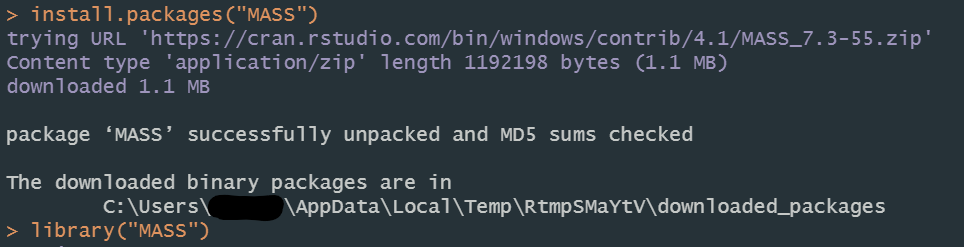
\includegraphics[width=\textwidth, keepaspectratio]{pakete.png}
    \end{center}
\end{frame}


\begin{frame}[fragile]{Empfehlenswerte Pakete}
	\begin{itemize}
		\item \verb+MatchIt+ für Propensity Score Matching 
	          \item \verb+MASS+ für Negativ-binomiale Regression \\
	          \item \verb+lmer+ bzw. \verb+lme4+ für Mixed-Models \\
	          \item \verb+pwr+ für Power-Analyse und insbesondere zur Fallzahlplanung \\
	          \item \verb+ggplot2+ für schöne Plots \\
	          \item \verb+haven+ für das Einlesen von \verb+.sav+-Dateien (SPSS) \\ 
	          \item ...
	\end{itemize}
\end{frame}
	



\end{document}
%% ================================================================== %%
%% ================================================================== %% 
